\documentclass{article}
\usepackage{graphicx} % Required for inserting images
\usepackage{amsmath}
\title{Threat hunting principles \\
}
\usepackage{array}
\author{Olof Magnusson}
\date{\today}
\begin{document}
	
	\maketitle
	
	\section*{What question are we trying to answer?}
Threat hunting is based on certain objectives that needs to be addressed. This essentially involves attempts to understand the threat actors objective, the cyber-terrain in which they operate and to identify how we can get closer to those objectives using well-defined searches in different SIEM-platforms. 



	\section*{Which data do you need for answering the question?}
	It is important to identify what type of data are required for each threat hunting exercise. There are certain circumstances where we might want to specify certain directories in which known bad actors operates. There may be data categories such as authentication, process, or firewall that need to be explicitly queried.
    
	\section*{How do you extract and validate that data?}
	The searches can be done in platforms such as \texttt{Microsoft Defender}, \texttt{Elastic} or \texttt{QRadar} depending on the objective of the threat actor. From the data, we can identify things that are legitimate, unknown, bad or interesting. The findings can then be exported in formats such as \textit{csv} to visualize the results and support documentation.
	\section*{What does the data tells you?}
	Analyzing the collected data to determine what belongs and what doesn't is a crucial part of this stage of the hunt. Framing questions like: \textit{How often does this process runs in this environment} or \textit{Why does this process only occurs at domain controllers} aids the analyst to look into the data in several different viewpoints.
	
	\section*{Conclude the threat hunting exercise}
	The conclusion involves writing a brief technical report outlining the steps taken to define the search terms and the types of findings identified. As indicated, the findings can be connected using the STIX framework in Figure \ref{STIX-framework} to illustrate relationships between data points.
		
		\begin{figure}[!htb]
			\centering
			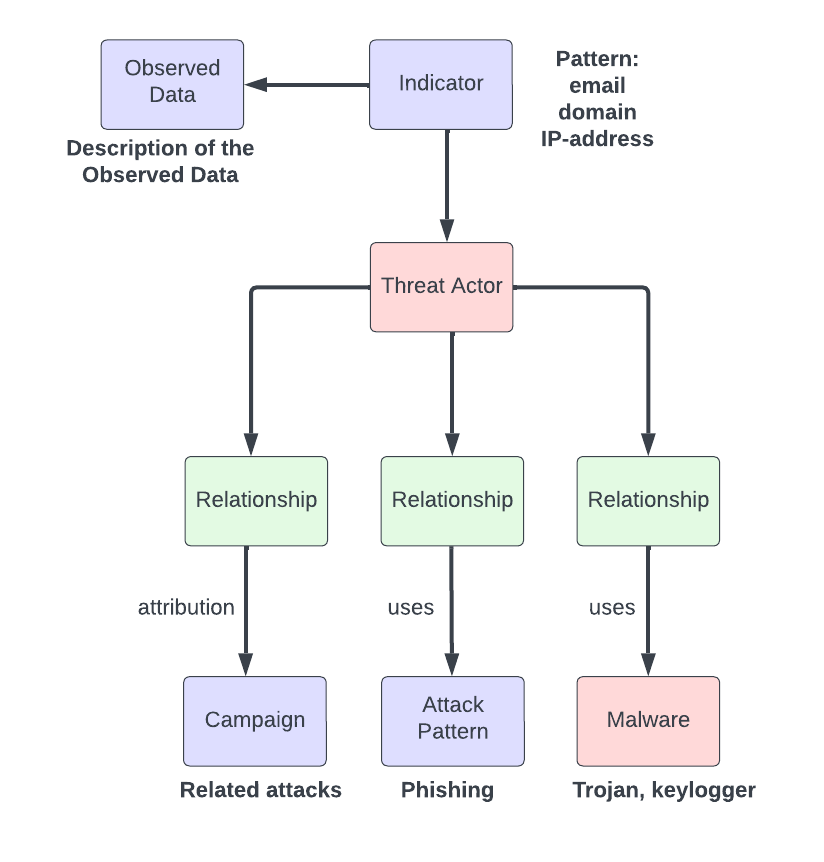
\includegraphics[width=\linewidth]{stix-test.png}
			\caption{STIX-framework}
			\label{STIX-framework}
		\end{figure}
	


\end{document}


